\chapter{Algorithms}
\label{C:Algorithms}

In this chapter we will describe the algorithms used in the experiements
in detail. We start by introducing the proposed algorithms \emph{MM} and 
\emph{MMC}, and continue with the reference algorithms used for 
comparison, \emph{Ratio}, \emph{Spectral} and \emph{Isomatch}.

\section{Proposed Matching Methods}
\label{S:MatchingMethods}

\subsection{Mirror Match (\emph{MM})}

\begin{figure}[h]
	\centering%
		\begin{subfigure}[t]{0.5\columnwidth}
			\centering
			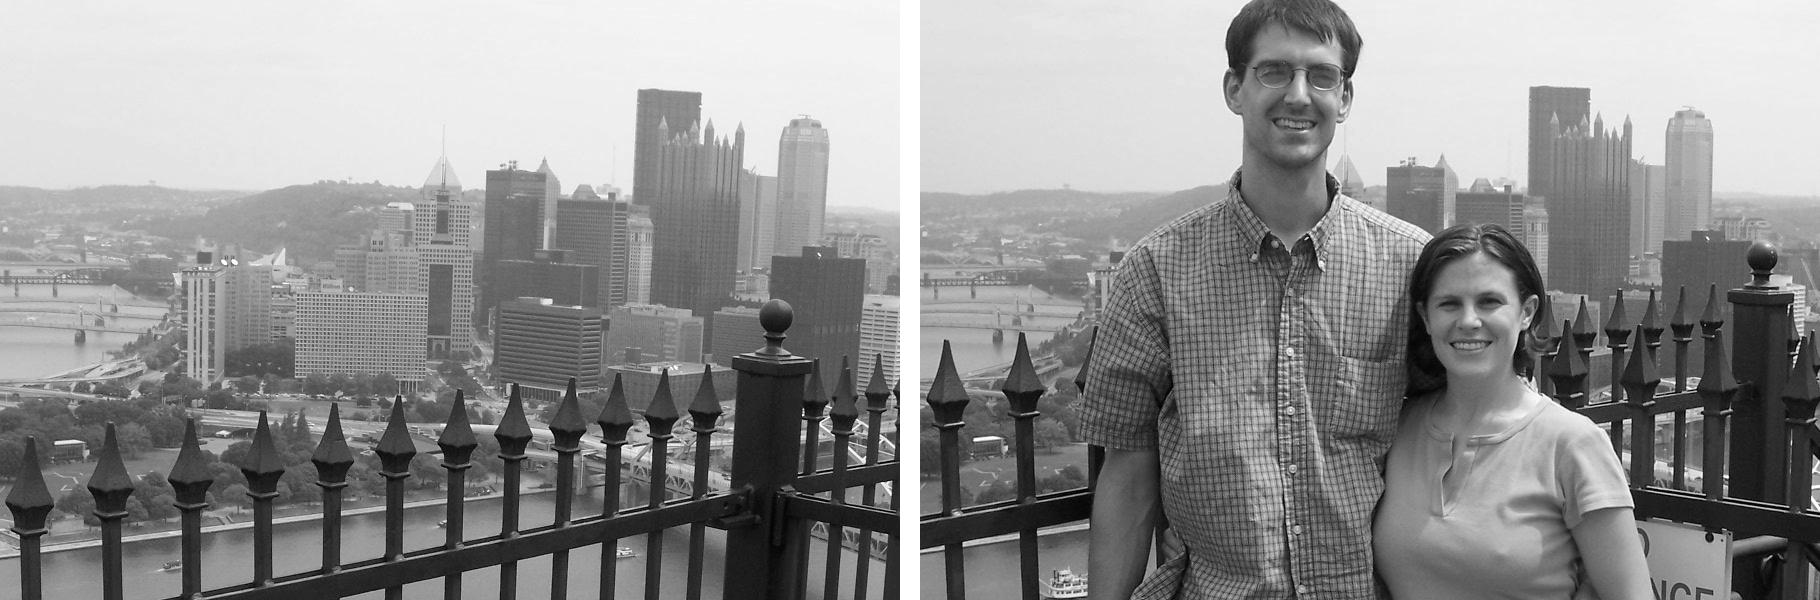
\includegraphics[width=0.95\columnwidth]{images/MMC_pitts_source}
			\caption{Source image pair}
			\label{fig:pitts_source}
		\end{subfigure}%
		~ %
		\begin{subfigure}[t]{0.5\columnwidth}
			\centering
			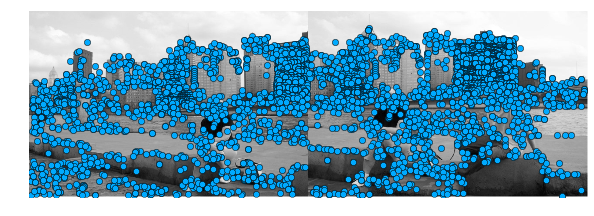
\includegraphics[width=0.95\columnwidth]{images/MMC_pitts_keypoints}
			\caption{Feature points}
			\label{fig:pitts_keypoints}
		\end{subfigure}%
		\\ %add desired spacing between images, e. g. ~, \quad, 
		%\qquad (or a blank line to force the subfigure onto a new line)
		\begin{subfigure}[t]{0.5\columnwidth}
			\centering
			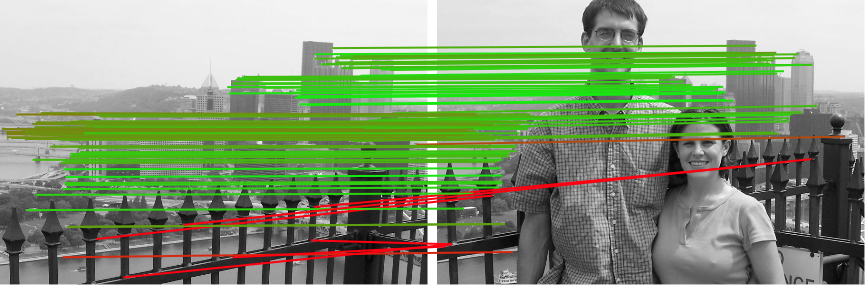
\includegraphics[width=0.95\columnwidth]{images/mirror_match_off}
			\caption{\emph{Ratio}}
			\label{fig:unique}
		\end{subfigure}%
		~ %add desired spacing between images, e. g. ~, \quad, 
		\begin{subfigure}[t]{0.5\columnwidth}
			\centering
			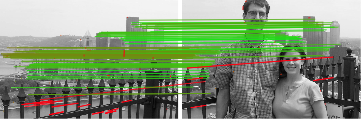
\includegraphics[width=0.95\columnwidth]{images/mirror_match_with_pruned}
			\caption{\emph{MM} intermediate result}
			\label{fig:within}
		\end{subfigure}%
		\\ %add desired spacing between images, e. g. ~, \quad, 
		%\qquad (or a blank line to force the subfigure onto a new line)
		\begin{subfigure}[t]{0.5\columnwidth}
			\centering
			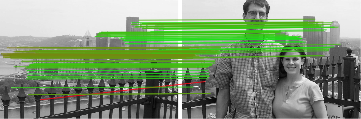
\includegraphics[width=0.95\columnwidth]{images/mirror_match}
			\caption{\emph{MM} final result}
			\label{fig:without}
		\end{subfigure}%
		~ %add desired spacing between images, e. g. ~, \quad, 
		\begin{subfigure}[t]{0.5\columnwidth}
			\centering
			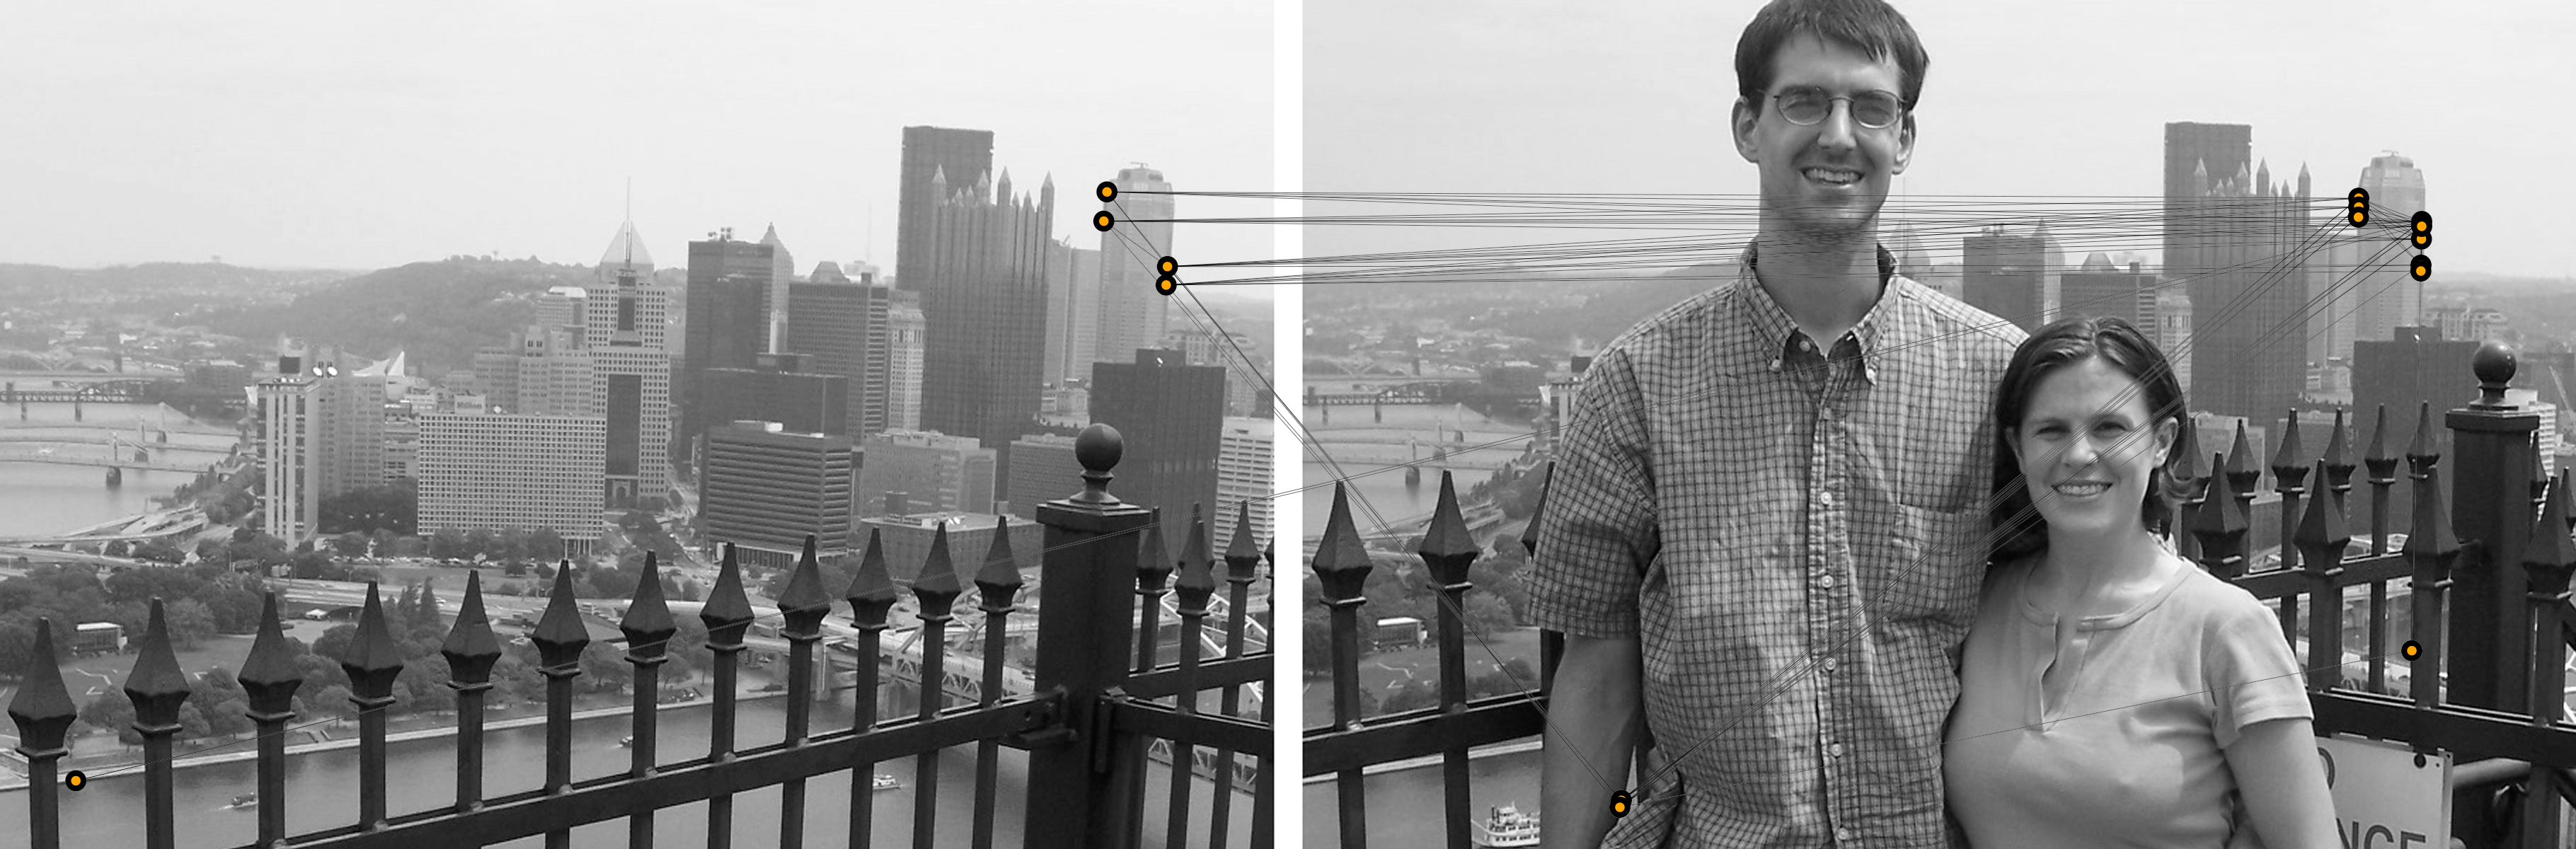
\includegraphics[width=0.95\columnwidth]{images/MMC_partition}
			\caption{\emph{MMC} Partition Example}
			\label{fig:pitts_partition}
		\end{subfigure}%
	\caption{Feature matching with \emph{MM} and \emph{MMC}. Dots represent feature points; green/red lines indicate correct/incorrect matches, respectively; black lines represent edges in the feature graph.  
	(c) Result of \emph{Ratio} matching. 
  (d) All matches found by \emph{MM}, including intra-image matches. 
	(e) Final \emph{MM} result. 
	(f) Example of a partition of feature points after clustering, which 
includes similar feature points from building windows and shirt patterns.}%
	\label{fig:comparemirror}%
\end{figure}%

The central idea behind \emph{MM} is to match features of $n$ images by 
taking every feature from all $n$ images and matching it against every 
other feature from the same set. We can then discard the correspondences 
that match two points within the same image. Algorithm~\ref{alg-mm} 
details the implementation of \emph{MM}.

\begin{algorithm}[htb]
\caption{Mirror Match (\emph{MM})}
\label{alg-mm}
%{\fontsize{10}{10}\selectfont
\begin{algorithmic}
\Require $images$ : set of images, $t \in \mathbb{R}$
\State $matches_{init}\gets \varnothing$
\State $matches_{final}\gets \varnothing$
\State $features\gets \varnothing$
\ForAll{$I_i \in images$} \Comment Acquisition Stage
	\State $features\gets features \cup getFeatures(I_i)$
\EndFor
\ForAll{$f_i \in features$} \Comment Matching Stage
	\State $f_m,f_n \gets get2NNs(f_i, features \setminus 
	\left\{f_i\right\})$
    \State $ratio \gets d(f_i, f_m) / d(f_i, f_n)$
	\If{$ratio < t$}
		\State $matches_{init} \gets matches_{init} \cup \left(f_i, f_m\right)$
	\EndIf
\EndFor
\ForAll{$\left(f_i, f_j \right) \in matches_{init}$} \Comment Filter 
Stage
\If{$\left(f_j, f_i \right) \in matches_{init} \wedge getImg(f_i) \neq 
getImg(f_j) \wedge \left(f_j, f_i\right) \not\in matches_{final}$}
		\State $matches_{final} \gets (f_i, f_j)$
	\EndIf
\EndFor \\
\Return $matches_{final}$
\end{algorithmic}
%}
\end{algorithm}

In the \emph{acquisition stage} we extract local feature points and 
obtain their descriptors from the set of images. The algorithm is not 
designed to make use of any feature extractor in particular, but for the
experiments (Chapter~\ref{C:Experiments}) the SIFT feature extractor and
descriptor has been used. In the \emph{matching} stage these features 
are matched using $k$-nearest neighbors.  The distance function $d(f_i, 
f_j)$ between features is calculated according to the feature 
descriptor. For SIFT we use the cosine similarity between the two 
descriptor vectors, while other descriptors might use other 
measures\footnote{BRIEF for example uses the hamming measure to speed up 
the computation}.  For any given feature $f_i$ the two closest neighbors 
are returned, and we calculate the ratio between them as proposed in 
\cite{lowe2004sift}\footnote{In Part~\ref{ss:ratio} this calculation and 
other details of \emph{Ratio} will be discussed}.  Any correspondence 
with a ratio above the threshold supplied will be discarded. Finally in 
the filter stage we check that matches are from different images and 
discard all matches that are not symmetric. That is; if a feature, 
$f_i$, is best matched to another feature, $f_j$, we would want for 
$f_j$ to be best matched to $f_i$ too.
This isn't always the case, for example if $f_i$ doesn't have a true 
correspondance in the other image, its closest neighbor $f_j$ might 
likely be better matched with a different feature point.

Figure~\ref{fig:comparemirror} illustrates the benefits of \emph{MM} 
using an example image pair from the Gallagher dataset 
\cite{gallagher2008}.
With \emph{Ratio} (Figure~\ref{fig:unique}), many incorrect matches occur 
in the fence towards the bottom of the image.
When we match all feature points together, many of these incorrect 
matches are eliminated, because points in the fence match with other 
points in the fence in the same image (Figures~\ref{fig:within} and
\ref{fig:without}).


\subsection{Mirror Match with Clustering (\emph{MMC})}

In contrast to \emph{MM}, \emph{MMC} diverges from traditional 
non-geometric feature matching by clustering feature points by 
similarity. This process yields partitions of similar feature points 
that we can match using the same approach as \emph{MM}.  
Algorithm~\ref{alg-mmc} shows the implementation of \emph{MMC}.

\begin{algorithm}[htb]
\caption{Mirror Match with Clustering (\emph{MMC})}
\label{alg-mmc}
%{\fontsize{10}{10}\selectfont
\begin{algorithmic}
\Require $images$ : set of images, $t \in \mathbb{R}$, $\alpha \in 
\mathbb{R}$
\State $M\gets \varnothing$
\State $F\gets \varnothing$
\ForAll{$I_i \in images$} \Comment Gather features
	\State $f_i\gets getFeatures(I_i)$
	\State $F\gets F \cup f_i$
\EndFor
\State $A\gets getAdjacencyMatrix(f_1, f_2,\; \ldots \;, f_n)$
\State $A_{norm}\gets normalize(A)$
\ForAll{$(i,j) \in indices(A)$} \Comment Prune edges
    \If{$A_{norm}[i,j] < \alpha$}
        \State $A_{norm}[i,j] \gets 0$
    \EndIf
\EndFor
\State $P\gets cluster(A_{norm})$
\ForAll{$p \in P$} \Comment p is a set of feature points
	\State $M\gets M \cup getMatches(p, t, F)$
\EndFor \\
\Return matches
\end{algorithmic}
%}
\end{algorithm}

To cluster the feature points, we construct a graph with the feature 
points as nodes and their similarity score as normalized edge weights.  
Given a set of $n$ features $F = {f_1, \ldots, f_n}$ and a similarity 
function $s$ we can define the matching function $M : (f_i, f_j) 
\rightarrow \mathbb{R}$ as follows:
\begin{equation*}
    M(a,b) = \begin{cases} s(f_i, f_j) & \mbox{if } f_i \neq f_j \\ 0 & 
    \mbox{otherwise}
	\end{cases}
\end{equation*}
The similarity function $s$ is based on the distance measure 
$d(f_i,f_j)$ (cosine similarity in the case of SIFT): $s(f_i, f_j) = 1 - 
d(f_i,f_j) / c$ where $c$ is a normalization constant normalizing the 
distance values between $0$ and $1$.
We obtain $A$, the normalized adjecency matrix of the fully connected 
similarity graph of feature points as follows:
\begin{equation*}
    A_{i,j} = \frac{M(f_i, f_j)}{\sum\limits_{f_i,f_j \in F} M(f_i, f_j) 
    / \left\vert F \right\vert ^ {2}}
\end{equation*}

In the literature there are various ways of clustering a graph according 
to different measures of what constitutes an optimal partitioning. 
Traditionally the most used clustering algorithms have been K-means and 
spectral clustering, but in recent years a host of new algorithms have 
been proposed based on both Newman's concept of graph 
modularity\footnote{Introduced in \cite{girvan2002}, discussed in 
\cite{brandes2007} and used in \cite{blondel2008} as well as others} as 
well as information theoretical measures\footnote{See for example 
\cite{rosvall2008}} and the Potts spin model from physics\footnote{Used 
in \cite{ronhovde2009}} just to mention a few. On tests done using 
randomly generated graphs with a known partitioning \cite{blondel2008}, 
\cite{rosvall2008} and \cite{ronhovde2009} perform markedly better than 
spectral clustering and K-means\cite{lancichinetti2009}.


\begin{figure}[t]
    \centering
	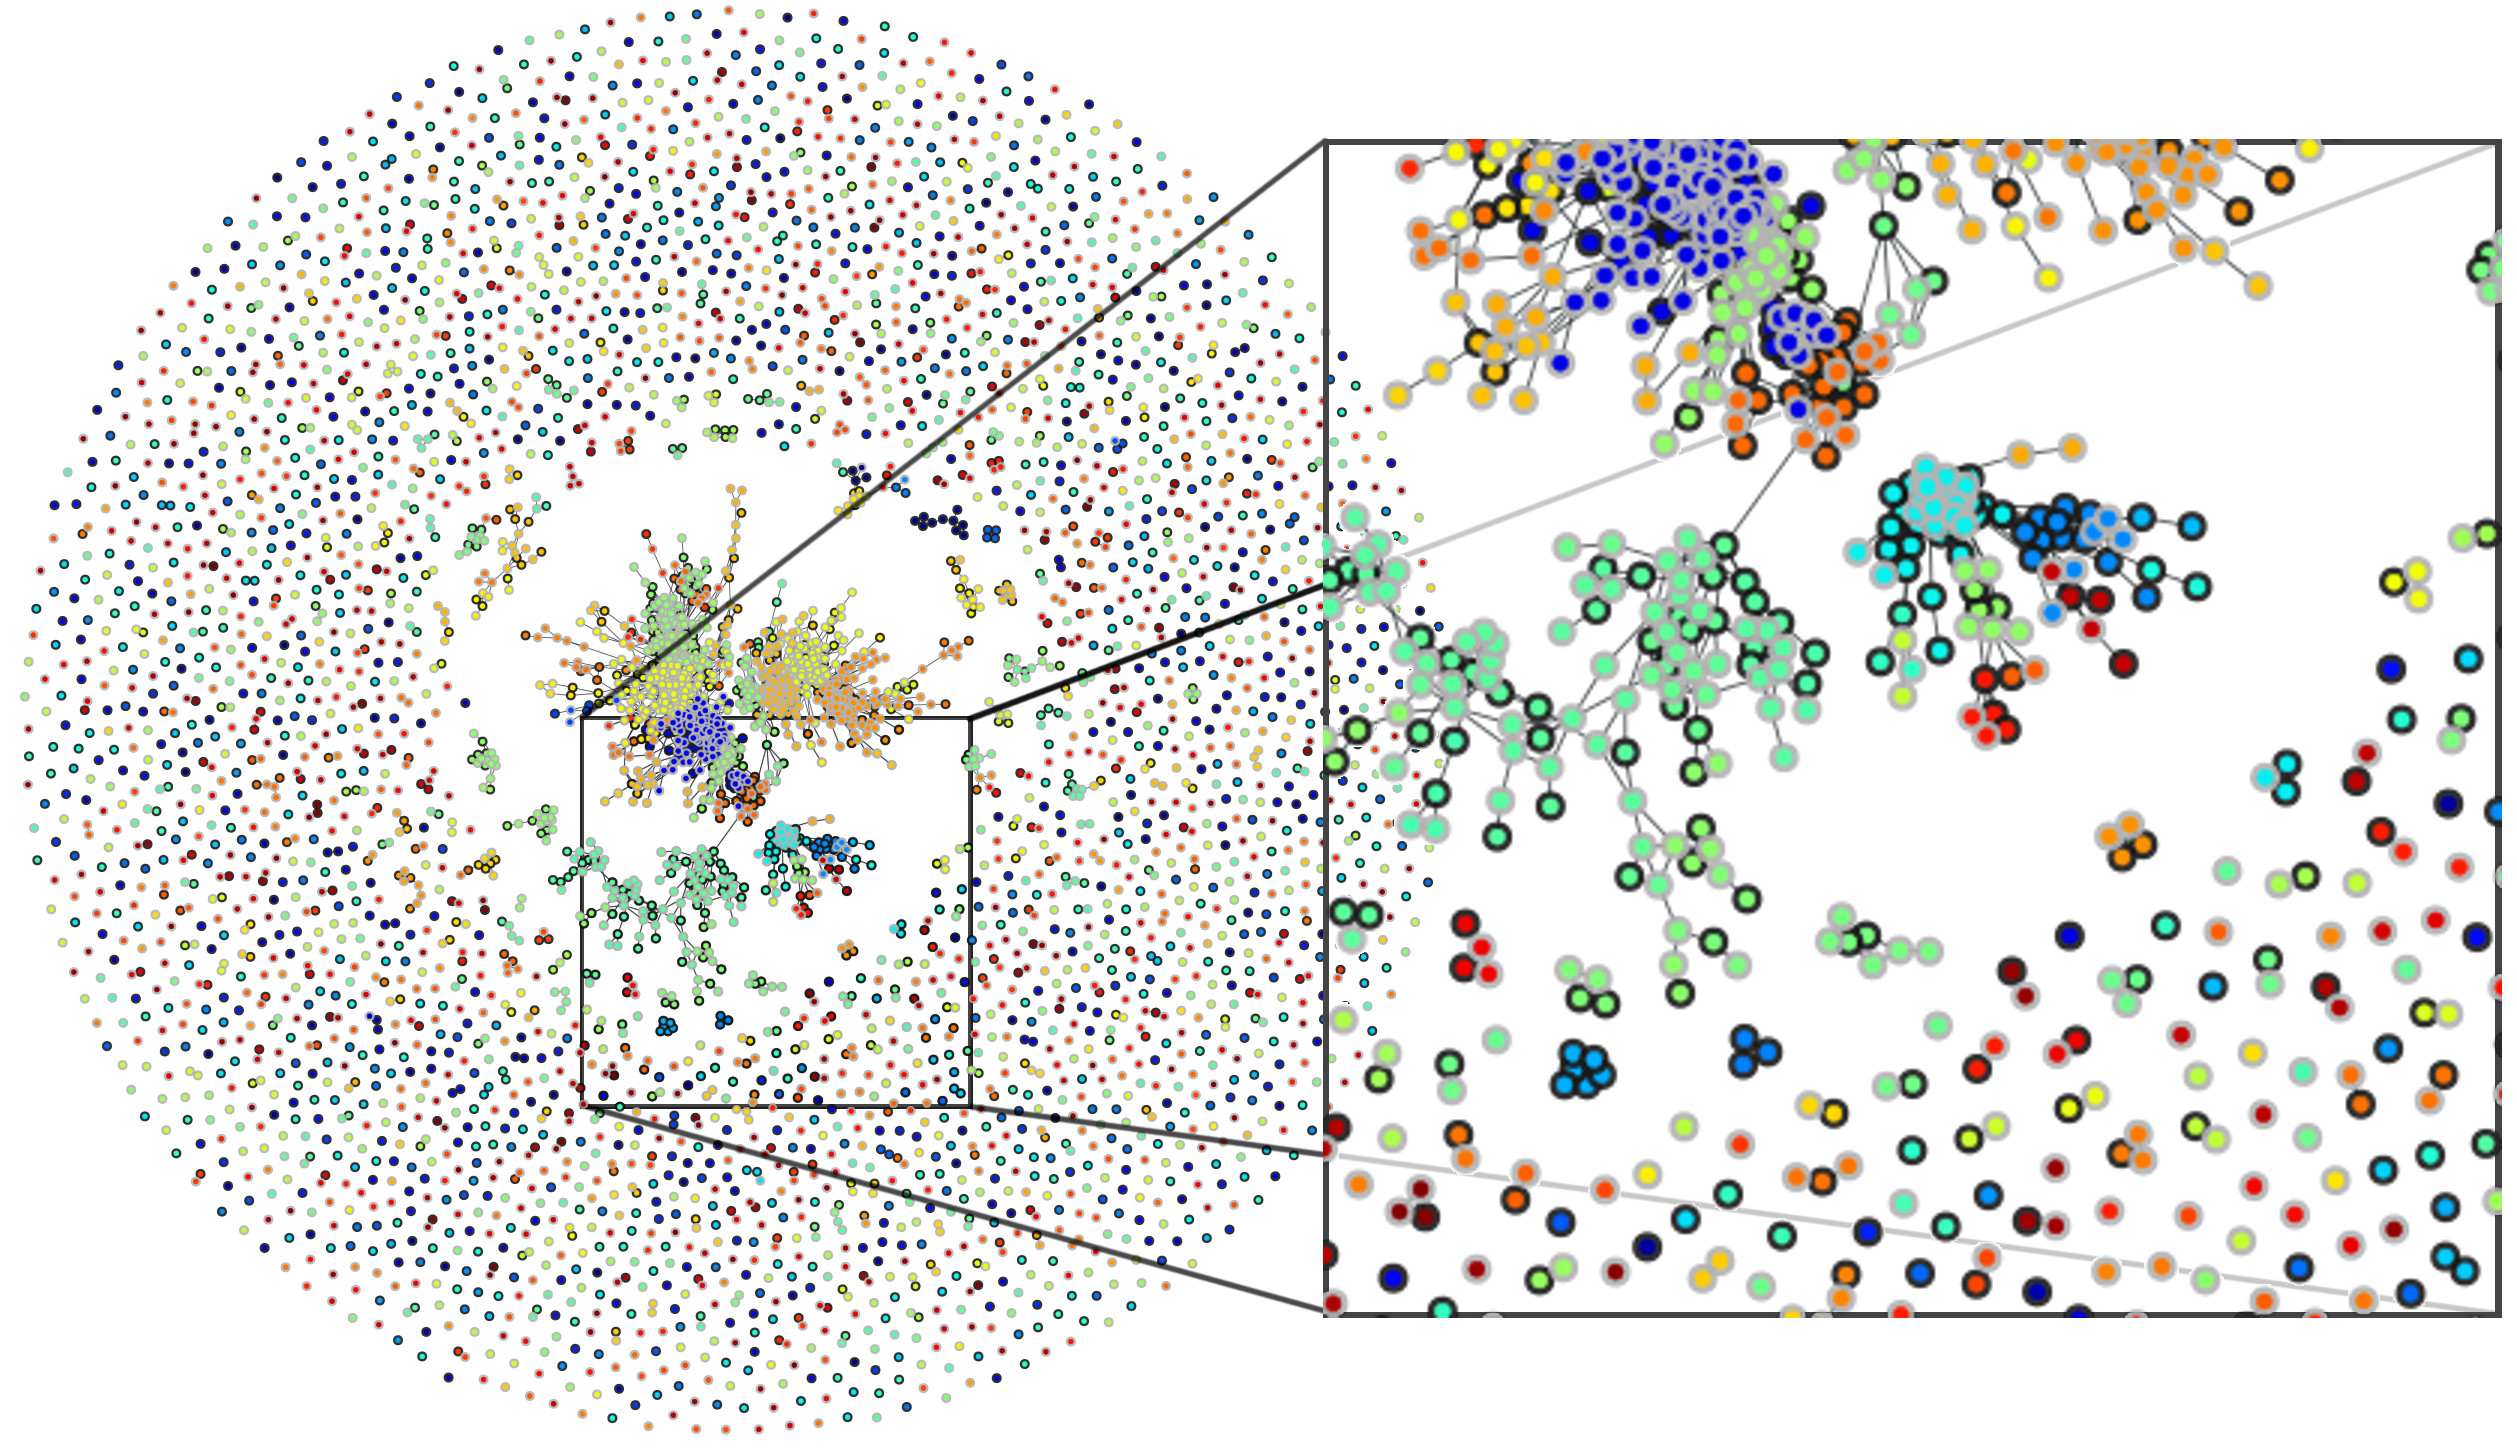
\includegraphics[width=\textwidth]{images/MMC_graph}
    \caption{The partitioned feature graph. Each vertex represents a 
        feature point; lines indicate high similarity between points. A 
        partition is a connected group with the same color. The border 
        color of each node indicates which image it belongs to.  Zooming 
    into a subsection of the graph (right part), the various cluster 
sizes can be seen, ranging from hundreds of feature points to only two 
or three.}
    \label{fig:graph-view}
\end{figure}

We use the Louvain Method \cite{blondel2008} for clustering feature 
points, since it is relatively fast and performs well 
\cite{lancichinetti2009}, does not require parameters 
\cite{blondel2008}, and does not emphasize partitions of equal size, as 
opposed to e.g.\ spectral clustering or k-means \cite{von2007}.

The louvain method is based on optimizing the \emph{Modularity} proposed 
by \cite{girvan2002} and defined as:
\begin{eqnarray*}
	Q & = & (\mbox{fraction of edges within communities}) \\
	  & & - (\mbox{expected fraction of such edges}) \\
	& = & \frac{1}{2m} \sum_{i,j} \left[ A_{ij} - \frac{k_i k_j}{2m} \
\right] \delta(c_i, c_j)
\end{eqnarray*}
Where $m=\frac{1}{2} \sum_{ij} A_{ij}$, $k_i = \sum_j A_{ij}$ and 
$A_{ij}$ is the weight between the edge connecting $i$ and $j$.  
$\delta(c_i, c_j)$ is the Kroneker Delta which is 1 only if the 
community assignment $c_i$ is equal to the community assignment $c_j$.

The Louvain Method is based on the maximizing the \emph{Modularity} of a 
graph iteratively. This is done efficiently because the gain in 
modularity from moving a vertex $v_i$ to a community $C$ can be 
calculated easily:
\begin{equation*}
	\Delta Q = \left[ \frac{\sum_{in} + 2 k_{i,in}}{2m} - \
    \left(\frac{\sum_{tot} + k_i}{2m} \right)^2 \right]
	- \left[\frac{\sum_{in}}{2m} - \left(\frac{\sum_{tot}}{2m} \
	\right)^2 - \left( \frac{k_i}{2m} \right)^2 \right]
\end{equation*}
Here as in the definition of \emph{Modularity}, $m=\frac{1}{2} \sum_{ij} 
A_{ij}$, $k_i = \sum_j A_{ij}$ and $k_{i,in}$ is the summed weights of 
the edges from $v_i$ to vertices in $C$.  $\sum_{in}$ is the sum of the 
weights of the edges of $C$ while $\sum_{tot}$ is the sum of all edges 
with at least one vertex in $C$.  The algorithm works by assigning each 
vertex to its proper cluster and then for each iteration reassign 
vertices to neighboring communities if it increases the 
\emph{Modularity}.  These iterations are carried out until there are no 
reassignments in which case an initial clustering has been reached.  For 
graphs consisting of a large number of vertices, the algorithm can now 
be repeated, treating each of the resulting clusters as a vertex and 
repeating the same procedure.

While the Louvain clustering algorithm does not require any parameters 
in itself, it tends towards clustering all feature points together in 
the same partition if the graph is very connected.  To ensure that the 
graph is well clustered, the adjacency matrix is pruned setting all 
edges below a certain threshold to $0$. In Algorithm~\ref{alg-mmc} this 
threshold is provided as the variable $\alpha$.  From empirical 
analysis, retaining the top 2.5\% of edges with the highest similarity 
seems to work well in practice. This requires estimating $\alpha$ 
parameter after obtaining the adjecency matrix.  
Figure~\ref{fig:graph-view} shows the result of clustering the feature 
points as a graph.

The partitions group feature points by similarity, which means that 
repetitive structures such as buildings often appear in larger 
partitions, as exemplified in Figure~\ref{fig:pitts_partition}.

\begin{algorithm}[htb]
\caption{Impl.\ of getMatches (\emph{from MMC algorithm})}
\label{alg-getmatches}
%\fontsize{10}{10}\selectfont
    \begin{algorithmic}
    \Require $p$ : set of features, $t\in \mathbb{R}$, $features$ : Set of 
    all features
    \State $edges \gets \left\{similarity(f_i, f_j) \mid getImg(f_i)
        \neq getImg(f_j) \wedge f_i, f_j \in p \right\}$
    \If{$\left\vert edges \right\vert > 1$}
        \State $matches \gets MMGet(p, t)$
    \ElsIf{$\left\vert edges \right\vert = 1$}
        \State $matches \gets RatioGet(p, features, t)$
    \Else
        \State $matches \gets \varnothing$
    \EndIf

    \Return matches
    \end{algorithmic}
\end{algorithm}

The matching algorithm for \emph{MMC} detailed in 
Algorithm~\ref{alg-getmatches} finds matches within all partitions with 
more than two elements using the \emph{MM} approach (\emph{MMGet}).  
However, as can be seen in the example in Figure~\ref{fig:graph-view}, 
many of the partitions contain only two feature points from different 
images linked by one edge. In this case, we compare the similarity of 
the these two feature points with their second best match and remove 
matches where this ratio lies above a certain threshold, like in the 
\emph{Ratio} algorithm (\emph{RatioGet}).  For example in the case of 
Figure~\ref{fig:pitts_partition}, we have feature points from a building 
in one image grouped together with points from a shirt pattern in 
another.  The nearest neighbor method would have returned wrong matches, 
but since we match the partition with \emph{MM}, points in the building 
end up matching other points in the building, and no matches are 
returned.

\section{The Competition}

The algorithms used in the comparison consists of two algorithms that 
use geometric data to enhance the matching, \emph{Isomatch} 
\cite{das2008event} and \emph{Spectral} \cite{leordeanu2005spectral} and 
one non geometric algorithm \emph{Ratio} \cite{lowe2004sift}.  
\emph{Ratio} is selected because it is a de facto standard for matching 
feature points, but also because it performs very well as shown by 
Mikolajczyk and Schmid in \cite{mikolajczyk2005performance}.  
\emph{Isomatch} and \emph{Spectral} on the other hand are selected 
because they are examples of two different approaches to geometric 
matching. \emph{Spectral} uses pairwise optimization to find a set of 
matches that is consistent in terms of direction and length which makes 
it less ideal in case of rotation and perspective change. 
\emph{Isomatch} focuses on matching only between geometric regions found 
by clustering the keypoints in the image.  This approach makes the 
algorithm resilient to rotation and perspective change, but will cause 
problems when the images matched are only partially overlapping and 
several regions do not have any corresponding regions in the other 
image.

\subsection{Ratio}
\label{ss:ratio}

\begin{algorithm}[htb]
\caption{Ratio Match (\emph{Ratio})}
\label{alg-ratio}
%{\fontsize{10}{10}\selectfont
\begin{algorithmic}
\Require $im_1$ : image, $im_2$ : image, $t \in \mathbb{R}$
\State $matches\gets \varnothing$
\State $features_1 \gets getFeatures(im_1)$
\State $features_2 \gets getFeatures(im_2)$
\ForAll{$f_i \in features_1$}
    \State $f_m,f_n \gets get2NNs(f_i, features_2)$
    \State $ratio \gets d(f_i, f_m) / d(f_i, f_n)$
	\If{$ratio < t$}
        \State $matches \gets \left(f_i, f_m\right)$
	\EndIf
\EndFor
\Return $matches$
\end{algorithmic}
%}
\end{algorithm}

\emph{Ratio} (Algorithm~\ref{alg-ratio}) \cite{lowe2004sift} diverges 
from from matching feature points by distance in that the metric we use 
to evaluate the feature points is the ratio of the distance to best 
match compared to the distance of the second best match. In detail, say 
$f_i$ is a feature point in an image $im_1$ and we are finding the 
closest match in another image $im_2$. Given the two closest neighbors 
to $f_i$ in in $im_l$, $f_m$ and $f_n$ ($d(f_i,f_m) < 
similarity(f_i,f_n)$ and a threshold $\beta$, we decide to return a 
match between $f_i$ and $f_j$ as follows:
\begin{equation*}
    match(f_i,(f_m,f_n)) = \begin{cases}
        \left\{(f_i,f_m)\right\} &
        \frac{d(f_i,f_m)}{d(f_i,f_n)} > \beta \\ \varnothing & 
        \mbox{otherwise}
    \end{cases}
\end{equation*}

We can call a distance measure \emph{Metric} given that it adheres to 
the following four properties: it is non-negative: $d(f_i,f_j) \geq 0$.  
It is only zero for identical inputs: $d(f_i,f_j) = 0 \Leftrightarrow 
f_i = f_j$. It is symmetric: $d(f_i,f_j) = d(f_j,f_i)$. It obeys the 
triangle inequality: $d(f_i,f_k) \leq d(f_i,f_j) + d(f_j,f_k)$.

This holds true for both cosine similarity and the hamming distance for 
which reason we can insert the feature points in a metric tree and 
retrieve the nearest neighbors in $O(log(n))$ computational time where 
$n$ is the amount of feature points.  Both \emph{Ratio} and \emph{MM} 
takes advantage of this property to match $n$ feature points in 
$O(nlog(n))$ computational time.


\subsection{Isomatch}

\begin{algorithm}[h]
\caption{Isomatch (\emph{Isomatch})}
\label{alg-isomatch}
%{\fontsize{10}{10}\selectfont
\begin{algorithmic}
\Require $im_1$ : image, $im_2$ : image, $t \in \mathbb{R}$
\State $matches_{init}\gets \varnothing$
\State $matches_{final}\gets \varnothing$
\State $features_1 \gets getFeatures(im_1)$
\State $features_2 \gets getFeatures(im_2)$
\ForAll{$f_i \in features_1$}
    \State $f_m,f_n \gets get2NNs(f_i, features_2)$
    \State $matches_{init} \gets \left(f_i, f_m\right)$
\EndFor
\State $partitions_1 \gets isodata(getPositions(features_1))$
\State $partitions_2 \gets isodata(getPositions(features_2))$
\State $P \gets getMatchMat(partitions_1, partitions_2, matches_{init})$
\ForAll{$(i,j) \in indices(P)$}
\If{$\left(P[i,j] > 5\right) \wedge \left(P[i,j] / sum(P_{i}) > 
0.5\right)$}
        \State $matches_{final} \gets getMatches(matches_{init}, 
        partitions_1, partitions_2, i, j)$
    \EndIf
\EndFor
\Return $matches_{final}$
\end{algorithmic}
%}
\end{algorithm}

\begin{figure}[htb]
	\centering
	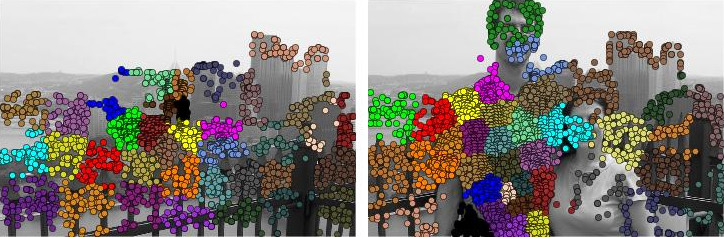
\includegraphics[width=\columnwidth]{images/isomatch_partitions}
	\caption{The result of partitioning feature points in two images.  
	Each dot represents a feature point and feature points grouped with 
the same color belong to the same partition.}
	\label{fig:isomatch_partitions}
\end{figure}

\emph{Isomatch} (Algorithm~\ref{alg-isomatch}) \cite{das2008event} is 
based on the idea that local feature points within a region in one image 
often matches to features within a corresponding region in the other 
image. To find these regions the algorithm uses the Isodata algorithm 
\cite{ball1965isodata} to perform unsupervised clustering on the 
positions of the feature points in the two images. This results in a 
fragmentation of the feature points into different regions based on 
their position in the image as demonstrated in 
Figure~\ref{fig:isomatch_partitions}. Based on this partitioning we 
create a correspondence matrix $P$. If we have $n$ regions in one image 
and $m$ regions in the other, $P$ is an $n \times m$ matrix. Given a set 
of matches $M = \{(f_{i,1}, f_{j}), \ldots \}$ and $n$ regions returned 
by Isodata, each region consisting of a set of feature points $R_i = 
\{f_i, f_j, \ldots\}$ we can construct $P$ as follows:
\begin{equation*}
    P_{i,j} = \sum_{(f_i,f_j) \in M} \delta_{f_i \in R_i}\delta_{f_j \in 
    R_j}
\end{equation*}
Here $\delta_{f_i \in R_i}$ is $1$ if $f_i \in R_i$ and $0$ otherwise.  
The initial set of matches are filtered based on $P$ by the $getMatches$ 
function. A match is kept only if it at least half the matches of the 
same region of origin also belong to the same region in the other image.  

The Isodata algorithm is similar to K-means with the addition that 
clusters are merged and split during the clustering process. In K-means 
we randomly assign the data points to $k$ clusters to begin with and 
calculate their mean. Then for each data point we reassign it to the 
cluster closest in mean. We then calculate the mean of the updated 
clusters and reiterate the process until we have spent a set amount of 
iterations or no reassignments have taken place. Isodata runs the same 
algorithm, but for each iteration it goes through the clusters and 
checks if any can be merged or split. Clusters are split if their 
variance along an axis is beyond a threshold, while two clusters are 
merged if their distance is below another threshold. This approach is 
beneficial when we don't know from the outside the amount of clusters we 
expect to see. For example in the case of feature points it is not 
obvious before clustering them regionally how many regions we obtain for 
an image.

To threshold the \emph{Isomatch} algorithm we filter the results using 
the ratio between first and second best match as in \emph{Ratio}, since 
\emph{Isomatch} itself doesn't readily admit any thresholding parameter.  

\subsection{Spectral}

\begin{algorithm}[h]
\caption{Spectral Match (\emph{Spectral})}
\label{alg-spectral}
%{\fontsize{10}{10}\selectfont
\begin{algorithmic}
\Require $im_1$ : image, $im_2$ : image, $t \in \mathbb{R}$
\State $matches_{init}\gets \varnothing$
\State $matches_{final} \gets \varnothing$
\State $features_1 \gets getFeatures(im_1)$
\State $features_2 \gets getFeatures(im_2)$
\ForAll{$f_i \in features_1$}
	\State $f_m,f_n \gets get2NNs(f_i, features_2)$
	\State $matches_{init} \gets \left(f_i, f_m\right)$
\EndFor
\State $M \gets matrix(\left\vert matches_{init} \right\vert, \left\vert 
matches_{init} \right\vert)$
\ForAll{$m_i \in matches_{init}$}
	\ForAll{$m_j \in matches_{init}$}
		\If{$i = j$}
			\State $M \gets matchSimilarity(m_i)$
		\Else
			\State $M \gets affinity(m_i, m_j)$
		\EndIf
	\EndFor
\EndFor
\State $x^{*} \gets maximumEigenvector(M)$
\ForAll{$\left(m_i, x_i\right) \in \left(matches_{init}, x^{*}\right)$}
	\If{$x_i > t$}
		\State $matches_{final} \gets matchtes_{final} \cup m_i$
	\EndIf
\EndFor

\Return $matches_{final}$
\end{algorithmic}
%}
\end{algorithm}

The \emph{Spectral} algorithm (Algorithm~\ref{alg-spectral}) used in the 
comparison of matching algorithms is based on the spectral matching 
algorithm proposed by Leordeanu and Herbert 
\cite{leordeanu2005spectral}.  The central idea behind it is that the 
set of actual correspondences of feature points between two images 
should be pairwise consistent. That is, given two feature points that 
are geometrically close in one image, for most cases we would assume 
that the closest correspondences of these two points in another image 
would be similarly close.  Based on this assumption we want to pick out 
a set of matches $T \subset S$ where $S$ is the initial set of possible 
matches such that the matches in $T$ are as pairwise consistent as 
possible. If we let $x$ be a binary vector corresponding in length to 
the set of initial matches $S$, where $x_i = 1$ if $m_i \subset T$, then 
we can formulate a subset-score as:
\begin{equation*}
	S = \sum_{m_i, m_j \in T} M(m_i, m_j) = x^TMx
\end{equation*}
The solution $x^{*}$ that maximizes this equation is then $x^{*} = 
argmax(x^TMx)$. By relaxing the constraints on $x$ such that it can take
values in the range of $\left[0, 1\right]$ we can interpret $x_i$ as the
association of $m_i$ with the optimal subset of matches $T$. Because we 
only worry about the relative values of $x$ we can fix the norm of $x$ 
to $1$, in which case by Raleigh's ratio theorem, the $x^{*}$ that 
optimizes $x^TMx$ is the principal eigenvector of $M$.

Leordeanu and Herbert proposes a simple affinity function to map the 
pairwise distance of two matches. In a scene where no rotation and 
excessive affine transformation takes place, it can generally be assumed 
that the length and direction of the vector between
the two feature points constituting the first match corresponds to the 
length and direction of the vector between the two feature points 
constituting the second match. Given two matches $m_i = (f_{i,1}, 
f_{i,2})$ and $m_j = (f_{j,1},f_{j,2})$ where $f_{k,n}$ is the feature 
point of match $k$ in image $n$, we denote the euclidean distance 
between feature points $f_{i,n}$ and $f_{j,n}$ in image $n$ as 
$d_{i,j,n}$.  The affinity function assigning a score based on the 
pairwise distance is then defined as follows:
\begin{equation*}
    M(a,b) = \begin{cases} 4.5 - \frac{\left(d_{i,j,1} - 
        d_{i,j,2}\right)^2}{2\sigma^2}, & \mbox{if } \left\vert 
                d_{i,j,1} - d_{i,j,2} \right\vert < 3\sigma \\ 0, & 
                \mbox{otherwise}
	\end{cases}
\end{equation*}
In the equation above $\sigma$ is a stabilizing parameter that controls 
the sensitivity of the score to deformations in the data. A larger 
$\sigma$ will allow for larger deformations. In the experiments it is 
fixed to 50. There are a number of occasions where the assumption that 
pairwise matches should have the same distance doesn't hold true.  A 
simple example would be matches between two images of the same scene 
where one image is rotated $180^{\circ}$.  However for a lot of 
applications like panorama stitching where we only see minor rotation 
and change of perspective the assumption is accurate.

In the implementation proposed by Leordeanu and Herbert 
\cite{leordeanu2005spectral} the last step of the algorithm greedily 
selects matches to ensure that matches are consistent, i.e.\ that two 
feature points in one image don't match with the same feature point in 
the other image. This is done by going through all the matches in the 
order of their associated $x^{*}$ score and for each match eliminating 
all matches in conflict with this match. This method ensure that as many
matches are kept as possible since only the conflicting matches are 
removed. However for cases where most feature points in one image will 
not have a correspondence in the other other image (e.g.\ cases of 
partial image overlap or object recognition) the greedy matching 
algorithm will keep finding matches even after the actual 
correspondences have already been found as long as they are consistent.

Since the testing is done on images with partial overlap, the final set 
of matches returned in Algorithm~\ref{alg-spectral} is the set of 
matches where the association of the match with the optimal subset of 
matches $T$ as measured by $x^{*}$ is above a certain threshold. For 
experiments the set of initial matches were given by the best match per 
feature point and the threshold was adjusted to allow for the best 50\% 
to be included in the set of final matches. A rate less than 50\% 
usually did not improve results, so to threshold the \emph{Spectral}
algorithm we filter the output using the ratio between first and second
best match as done in \emph{Ratio}.
